% ============================================================
% SEMINAR SLIDE: Hybrid Search — Theory & Practice
% LaTeX Beamer — Knowledge Deep-Dive (10–15 phút)
% ============================================================
\documentclass[aspectratio=169, 11pt]{beamer}

% ---- Encoding & Language ----
\usepackage[utf8]{inputenc}
\usepackage[T5]{fontenc}
\usepackage{vietnam}

% ---- Theme & Colors ----
\usetheme{Madrid}
\usecolortheme{default}

% ── Color palette (improved contrast) ──
\definecolor{primaryDark}{HTML}{0F1B2D}
\definecolor{primaryMid}{HTML}{172640}
\definecolor{accentTeal}{HTML}{2DD4BF}      % brighter teal
\definecolor{accentBlue}{HTML}{60A5FA}      % brighter blue
\definecolor{accentOrange}{HTML}{FB923C}    % softer orange
\definecolor{accentPurple}{HTML}{A78BFA}    % brighter purple
\definecolor{accentRed}{HTML}{F87171}       % for alerts
\definecolor{textWhite}{HTML}{F1F5F9}      % near-white
\definecolor{textLight}{HTML}{CBD5E1}       % readable secondary
\definecolor{textMuted}{HTML}{94A3B8}       % subtle but visible
\definecolor{boxBg}{HTML}{1E293B}
\definecolor{highlightRow}{HTML}{134E4A}    % dark teal for row highlight
\definecolor{codeGreen}{HTML}{6EE7B7}
\definecolor{codePurple}{HTML}{C4B5FD}
\definecolor{codeYellow}{HTML}{FDE68A}

% ── Apply dark theme ──
\setbeamercolor{normal text}{fg=textWhite, bg=primaryDark}
\setbeamercolor{structure}{fg=accentTeal}
\setbeamercolor{title}{fg=white, bg=primaryMid}
\setbeamercolor{frametitle}{fg=white, bg=primaryMid}
\setbeamercolor{block title}{fg=white, bg=accentBlue!80!black}
\setbeamercolor{block body}{fg=textWhite, bg=boxBg}
\setbeamercolor{block title alerted}{fg=white, bg=accentRed!80!black}
\setbeamercolor{block body alerted}{fg=textWhite, bg=boxBg}
\setbeamercolor{block title example}{fg=white, bg=accentTeal!70!black}
\setbeamercolor{block body example}{fg=textWhite, bg=boxBg}
\setbeamercolor{itemize item}{fg=accentTeal}
\setbeamercolor{itemize subitem}{fg=accentBlue}
\setbeamercolor{enumerate item}{fg=accentTeal}
\setbeamercolor{footline}{fg=textMuted, bg=primaryMid}
\setbeamercolor{page number in head/foot}{fg=textMuted}
\setbeamercolor{author in head/foot}{fg=textMuted}
\setbeamercolor{title in head/foot}{fg=accentTeal}

\setbeamerfont{title}{size=\Large, series=\bfseries}
\setbeamerfont{frametitle}{size=\large, series=\bfseries}
\setbeamerfont{block title}{size=\normalsize, series=\bfseries}
\setbeamerfont{section head}{size=\scriptsize, series=\mdseries}
\setbeamertemplate{navigation symbols}{}

% Redefine frametitle to display current section on the right
\setbeamertemplate{frametitle}{%
  \nointerlineskip
  \begin{beamercolorbox}[wd=\paperwidth,ht=3ex,dp=1.5ex,leftskip=0.5cm,rightskip=0.5cm]{frametitle}%
    \usebeamerfont{frametitle}\insertframetitle%
    \hfill\usebeamerfont{section head}\textcolor{accentTeal}{\insertsectionhead}%
  \end{beamercolorbox}%
}

% ---- Packages ----
\usepackage{amsmath, amssymb}
\usepackage{graphicx}
\graphicspath{{./}{../Report_Final/images/}}
\usepackage{tikz}
\usetikzlibrary{arrows.meta, positioning, shapes.geometric, calc, backgrounds, fit}
\usepackage{listings}
\usepackage{booktabs}
\usepackage{multirow}
\usepackage{hyperref}
\usepackage{array}
\usepackage{colortbl}

% Code listing style
\lstdefinestyle{codestyle}{
    basicstyle=\ttfamily\scriptsize\color{textWhite},
    keywordstyle=\color{codePurple}\bfseries,
    stringstyle=\color{codeGreen},
    commentstyle=\color{textMuted}\itshape,
    backgroundcolor=\color{primaryMid},
    frame=single,
    rulecolor=\color{accentTeal!40},
    breaklines=true,
    showstringspaces=false,
    tabsize=2,
}
\lstset{style=codestyle}

% ---- Metadata ----
\title[Hybrid Search]{Hybrid Search}
\subtitle{Kết hợp Keyword Search, Semantic Search\\và Reciprocal Rank Fusion}
\author[Group 11]{
  \texorpdfstring{
    \textbf{Instructor(s):} PGS.TS Thoai Nam\\[0.2cm]
    \textbf{Student(s):}\\
    {\small
    Duong Gia An --- 2470293 \quad
    Trinh Son Lam --- 2470287 \quad
    Nguyen Thanh Huyen --- 2570416
    }
  }{Duong Gia An, Trinh Son Lam, Nguyen Thanh Huyen}
}
\institute[HCMUT]{
    Đại học Bách khoa TP.HCM --- Khoa KH \& KT Máy tính\\
    CO5135 --- Big Data (HK252)
}
\date{Tháng 5, 2026}
\titlegraphic{
\includegraphics[height=1.2cm]{hcmut.png}}

% ============================================================
\begin{document}

% ── SLIDE 1: Title ──
\begin{frame}[plain]
    \begin{center}
        \vspace*{0.1cm}
        
\includegraphics[height=1.1cm]{hcmut.png}
        \vspace*{0.25cm}
        
        % Đóng khung cả tên seminar và phần tiếng Việt phụ đề
        {\color{accentTeal}\setlength{\fboxrule}{1.2pt}\setlength{\fboxsep}{10pt}\fbox{%
            \begin{minipage}{0.75\textwidth}
                \centering
                {\LARGE \bfseries HYBRID SEARCH}
                
                \vspace*{0.15cm}
                {\large \color{textWhite} Kết hợp Keyword Search, Semantic Search\\và Reciprocal Rank Fusion}
            \end{minipage}%
        }}
    \end{center}
    
    \vspace*{0.15cm}
    
    % Góc phải giữa: Tên giảng viên & sinh viên
    \begin{flushright}
        {\footnotesize \color{textLight}
        \begin{tabular}{r}
            \textcolor{textMuted}{Instructor(s):} PGS.TS Thoai Nam \\[0.12cm]
            \textcolor{textMuted}{Student(s):} \\
            Duong Gia An --- 2470293 \\
            Trinh Son Lam --- 2470287 \\
            Nguyen Thanh Huyen --- 2570416
        \end{tabular}
        \hspace*{0.5cm}
        }
    \end{flushright}
    
    \vspace*{\fill}
    
    % Dưới cùng: Thông tin trường, khoa, môn học và ngày tháng
    \begin{center}
        {\scriptsize \color{textMuted}
        Đại học Bách khoa TP.HCM --- Khoa KH \& KT Máy tính --- CO5135 --- Big Data (HK252) \\
        Tháng 5, 2026
        }
    \end{center}
\end{frame}

% ── SLIDE 2: TOC ──
\begin{frame}{Nội dung trình bày}
\begin{columns}[T]
\begin{column}{0.48\textwidth}
\tableofcontents[sections={1-3}]
\end{column}
\begin{column}{0.48\textwidth}
\tableofcontents[sections={4-6}]
\end{column}
\end{columns}
\end{frame}

% ============================================================
% SECTION 1
% ============================================================
\section{Bài toán tìm kiếm (Information Retrieval)}

\begin{frame}{Sự bùng nổ dữ liệu phi cấu trúc}
\begin{columns}[T]
\begin{column}{0.52\textwidth}

\begin{alertblock}{Thực trạng}
{\small Mỗi ngày thế giới tạo ra \textbf{2.5 quintillion bytes} dữ liệu. Phần lớn là \textbf{phi cấu trúc}: văn bản, ảnh, video, bài báo...}
\end{alertblock}

\vspace{0.2cm}

\textbf{Các kho dữ liệu lớn:}
\begin{itemize}
    \item \textcolor{accentBlue}{\textbf{Google}}: 130+ nghìn tỷ trang web
    \item \textcolor{accentOrange}{\textbf{arXiv}}: 2.4+ triệu bài báo
    \item \textcolor{accentPurple}{\textbf{Wikipedia}}: 60+ triệu bài viết
\end{itemize}

\vspace{0.1cm}
{\small $\Rightarrow$ \textbf{Information Retrieval (IR)}: tìm kiếm thông tin liên quan trong dữ liệu lớn.}

\end{column}
\begin{column}{0.45\textwidth}

\begin{block}{IR Pipeline chuẩn}
{\small
\begin{enumerate}
    \item \textbf{Ingestion}: Thu thập, làm sạch
    \item \textbf{Indexing}: Cấu trúc tra cứu nhanh
    \item \textbf{Retrieval}: Nhận query, xếp hạng
\end{enumerate}
}
\end{block}

\vspace{0.2cm}

\begin{exampleblock}{Ba thế hệ tìm kiếm}
\begin{enumerate}
    \item \textcolor{accentBlue}{\textbf{Lexical}} (1970s): Đối khớp từ khóa
    \item \textcolor{accentOrange}{\textbf{Semantic}} (2018): Hiểu ngữ nghĩa (AI)
    \item[\textcolor{accentTeal}{$\star$}] \textcolor{accentTeal}{\textbf{Hybrid}} (2022+): Kết hợp cả hai!
\end{enumerate}
\end{exampleblock}

\end{column}
\end{columns}
\end{frame}

% ============================================================
% SECTION 2
% ============================================================
\section{Tìm kiếm từ khóa (Keyword Search)}

\begin{frame}{Inverted Index --- Nền tảng mọi Search Engine}
\begin{columns}[T]
\begin{column}{0.46\textwidth}

\textbf{Ý tưởng:} Thay vì quét toàn bộ tài liệu, xây dựng \textbf{bảng tra cứu ngược}:

\vspace{0.3cm}

\begin{block}{Forward Index {\small (quét tuần tự)}}
\centering
{\small
\begin{tabular}{l|l}
\textcolor{accentTeal}{\textbf{Doc}} & \textcolor{accentTeal}{\textbf{Nội dung}} \\
\hline
$D_1$ & deep learning for NLP \\
$D_2$ & deep neural networks \\
$D_3$ & NLP with transformers \\
\end{tabular}
}

\vspace{0.15cm}
{\small\textcolor{textLight}{$\to$ Quét tuần tự $\to$ $O(N)$}}
\end{block}

\end{column}
\begin{column}{0.50\textwidth}

\begin{exampleblock}{Inverted Index {\small (tra ngược)}}
\centering
{\small
\begin{tabular}{l|l}
\textcolor{accentTeal}{\textbf{Term}} & \textcolor{accentTeal}{\textbf{Posting List}} \\
\hline
deep & $[D_1, D_2]$ \\
learning & $[D_1]$ \\
NLP & $[D_1, D_3]$ \\
neural & $[D_2]$ \\
transformers & $[D_3]$ \\
\end{tabular}
}

\vspace{0.15cm}
{\small\textcolor{accentTeal}{$\to$ Tra bảng ngay $\to$ $O(1)$ lookup!}}
\end{exampleblock}

\vspace{0.3cm}
\textbf{Ai dùng?}\\
{\small Google, Elasticsearch, Apache Solr, Lucene, Bing, Wikipedia, Stack Overflow...}

\end{column}
\end{columns}
\end{frame}

% ── BM25 ──
\begin{frame}[fragile]{BM25 --- Thuật toán xếp hạng chuẩn}

\begin{block}{Công thức BM25 {\scriptsize (Robertson \& Zaragoza, 2009)}}
\vspace{-0.15cm}
\[
\text{BM25}(D, Q) = \sum_{i=1}^{n} \underbrace{\text{IDF}(q_i)}_{\text{Từ hiếm}\to\text{quan trọng}} \cdot \frac{\overbrace{f(q_i, D)}^{\text{Term Freq}} \cdot (k_1 + 1)}{f(q_i, D) + k_1 \cdot \left(1 - b + b \cdot \frac{|D|}{\text{avgdl}}\right)}
\]
\vspace{-0.15cm}
\end{block}

\begin{columns}[T]
\begin{column}{0.46\textwidth}
{\scriptsize
\textbf{Ba yếu tố quyết định:}
\begin{itemize}
    \item \textcolor{accentBlue}{\textbf{TF}}: Xuất hiện nhiều $\to$ bão hòa
    \item \textcolor{accentOrange}{\textbf{IDF}}: Từ hiếm $\to$ trọng số cao. VD: ``transformer'' $\gg$ ``the''
    \item \textcolor{accentPurple}{\textbf{Doc Length}}: Tài liệu dài bị phạt
\end{itemize}
Tham số chuẩn: $k_1 = 1.2$, $b = 0.75$
}
\end{column}
\begin{column}{0.50\textwidth}

\begin{exampleblock}{Dùng ở đâu?}
{\scriptsize ES, OpenSearch, Solr, Lucene, SQLite FTS5. Mặc định cho keyword search.}
\end{exampleblock}

\begin{alertblock}{Hạn chế cốt lõi}
{\scriptsize BM25 chỉ hiểu \textbf{từ vựng}, không hiểu \textbf{ngữ nghĩa}:
\begin{itemize}
    \item ``car'' $\neq$ ``automobile''
    \item ``detect fake images'' $\neq$ ``deepfake''
\end{itemize}
}
\end{alertblock}
\end{column}
\end{columns}
\end{frame}

% ============================================================
% SECTION 3
% ============================================================
\section{Tìm kiếm ngữ nghĩa (Semantic Search)}

\begin{frame}{Vector Embedding --- Từ ngôn ngữ đến toán học}
\begin{columns}[T]
\begin{column}{0.53\textwidth}

\textbf{Ý tưởng:} Biểu diễn \textit{ý nghĩa} văn bản bằng vector. Các văn bản tương đồng ngữ nghĩa $\to$ vector \textbf{gần nhau}.

\vspace{0.1cm}

\begin{block}{Lịch sử phát triển}
{\small
\begin{enumerate}
    \item \textbf{Word2Vec} (2013): Mỗi \textit{từ} $\to$ 1 vector.
    \item \textbf{BERT} (2018): Hiểu \textit{ngữ cảnh}. ``bank'' (ngân hàng) $\neq$ ``bank'' (bờ sông)
    \item \textbf{Sentence Transformers} (2019): Mỗi \textit{câu} $\to$ 1 vector. Tối ưu cho search.
\end{enumerate}
}
\end{block}

\vspace{0.1cm}
\textbf{Cosine Similarity:}
$\;\cos(\vec{a}, \vec{b}) = \dfrac{\vec{a} \cdot \vec{b}}{\|\vec{a}\| \cdot \|\vec{b}\|} \in [-1, 1]$

\end{column}
\begin{column}{0.44\textwidth}

% Vector space
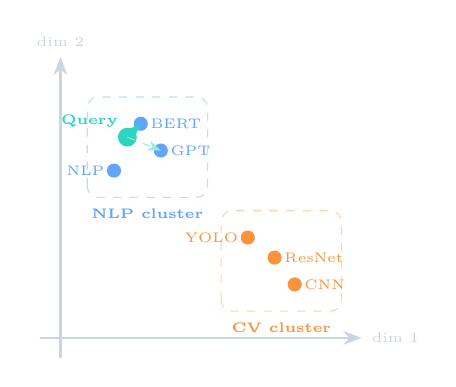
\begin{tikzpicture}[scale=0.85]
    \draw[-{Stealth}, thick, textLight] (-0.3,0) -- (4.5,0) node[right, font=\tiny, text=textLight] {dim 1};
    \draw[-{Stealth}, thick, textLight] (0,-0.3) -- (0,4.2) node[above, font=\tiny, text=textLight] {dim 2};
    
    \fill[accentBlue] (1.2, 3.2) circle (3pt) node[right, font=\tiny, text=accentBlue] {BERT};
    \fill[accentBlue] (1.5, 2.8) circle (3pt) node[right, font=\tiny, text=accentBlue] {GPT};
    \fill[accentBlue] (0.8, 2.5) circle (3pt) node[left, font=\tiny, text=accentBlue] {NLP};
    \draw[accentBlue!40, dashed, rounded corners] (0.4, 2.1) rectangle (2.2, 3.6);
    \node[font=\tiny\bfseries, text=accentBlue] at (1.3, 1.85) {NLP cluster};
    
    \fill[accentOrange] (3.2, 1.2) circle (3pt) node[right, font=\tiny, text=accentOrange] {ResNet};
    \fill[accentOrange] (3.5, 0.8) circle (3pt) node[right, font=\tiny, text=accentOrange] {CNN};
    \fill[accentOrange] (2.8, 1.5) circle (3pt) node[left, font=\tiny, text=accentOrange] {YOLO};
    \draw[accentOrange!40, dashed, rounded corners] (2.4, 0.4) rectangle (4.2, 1.9);
    \node[font=\tiny\bfseries, text=accentOrange] at (3.3, 0.15) {CV cluster};
    
    \fill[accentTeal] (1.0, 3.0) circle (4pt);
    \node[font=\tiny\bfseries, text=accentTeal, above left] at (1.0, 3.0) {Query};
    \draw[-{Stealth}, accentTeal, thick, dashed] (1.0, 3.0) -- (1.2, 3.2);
    \draw[-{Stealth}, accentTeal!50, dashed] (1.0, 3.0) -- (1.5, 2.8);
\end{tikzpicture}

\vspace{0.2cm}

\begin{exampleblock}{Ứng dụng thực tế}
{\small Google Search, Spotify (gợi nhạc), Netflix, Airbnb, RAG pipelines (ChatGPT + retrieval)}
\end{exampleblock}

\end{column}
\end{columns}
\end{frame}

% ── Models ──
\begin{frame}{Embedding Models \& Cosine Similarity}
\begin{columns}[T]
\begin{column}{0.50\textwidth}

\begin{block}{Embedding Models phổ biến}
\centering
\renewcommand{\arraystretch}{0.9}
{\small
\begin{tabular}{l c c l}
\toprule
\textbf{Model} & \textbf{Dims} & \textbf{MTEB} & \textbf{Ghi chú} \\
\midrule
MiniLM-L6-v2 & 384 & 56 & Nhẹ, nhanh \\
bge-small-v1.5 & 384 & 62 & BAAI \\
e5-large-v2 & 1024 & 64 & Microsoft \\
text-embed-3-large & 3072 & 65 & OpenAI API \\
SPECTER2 & 768 & --- & Academic \\
\bottomrule
\end{tabular}
}
\end{block}

\end{column}
\begin{column}{0.46\textwidth}

\begin{exampleblock}{Cosine Similarity thực tế}
\centering
\renewcommand{\arraystretch}{0.9}
{\small
\begin{tabular}{l c}
\toprule
\textbf{Cặp câu} & \textbf{Cosine} \\
\midrule
fake images $\leftrightarrow$ image forgery & \textcolor{accentTeal}{\textbf{0.70}} \\
car $\leftrightarrow$ automobile & \textcolor{accentTeal}{0.78} \\
bank (tiền) $\leftrightarrow$ bank (sông) & \textcolor{accentRed}{0.35} \\
\bottomrule
\end{tabular}
}
\end{exampleblock}

\vspace{0.15cm}
\textbf{Đặc trưng cốt lõi:}
\begin{itemize}
    \item {\small \textbf{Trade-off}: Kích thước vector lớn $\to$ biểu diễn ngữ nghĩa tốt hơn nhưng tốn RAM và băng thông.}
    \item {\small \textbf{MTEB}: Bảng xếp hạng chuẩn đánh giá chất lượng mô hình nhúng.}
\end{itemize}

\end{column}
\end{columns}
\end{frame}

\begin{frame}{Tìm kiếm chính xác vs Tìm kiếm xấp xỉ}
\begin{columns}[T]
\begin{column}{0.48\textwidth}

\begin{alertblock}{Tìm kiếm chính xác: $O(N \cdot d)$ quá chậm!}
{\small $N{=}1M$ văn bản, $d{=}384$ chiều $\to$ \textbf{384 triệu phép tính} cho mỗi truy vấn!}
\begin{itemize}
    \item Phép quét tuyến tính (Exact brute-force kNN)
    \item Không khả thi đối với dữ liệu lớn (Big Data)
\end{itemize}
\end{alertblock}

\begin{block}{Giải pháp: Tìm kiếm xấp xỉ (ANN)}
{\small Chấp nhận kết quả láng giềng gần đúng để đổi lấy tốc độ truy xuất cực nhanh ($O(N) \to O(\log N)$).}
\end{block}

\end{column}
\begin{column}{0.48\textwidth}

\begin{block}{Các thuật toán tìm kiếm xấp xỉ}
\centering
\renewcommand{\arraystretch}{0.9}
{\small
\begin{tabular}{l l l}
\toprule
\textbf{Thuật toán} & \textbf{Ý tưởng} & \textbf{Dùng bởi} \\
\midrule
\textbf{LSH} & Hash function & Uber \\
\textbf{IVF} & K-Means clusters & FAISS (Meta) \\
\textbf{HNSW} & Đồ thị đa tầng & Elasticsearch \\
\textbf{ScaNN} & Quantization & Google \\
\bottomrule
\end{tabular}
}
\end{block}

\vspace{0.1cm}

\textbf{HNSW} {\small (Malkov \& Yashunin, 2018):}
\begin{itemize}
    \item {\small Đồ thị đa tầng tương tự Skip List: lớp trên nhảy xa định vị nhanh, lớp dưới chi tiết dần.}
    \item {\small Dùng mặc định trong Elasticsearch, Pinecone, Qdrant.}
\end{itemize}

\end{column}
\end{columns}
\end{frame}

% ============================================================
% SECTION 4
% ============================================================
\section{Tìm kiếm kết hợp (Hybrid Search)}

\begin{frame}{Tại sao cần Hybrid Search?}
\begin{columns}[T]
\begin{column}{0.46\textwidth}

\begin{block}{\textcolor{accentBlue}{Tìm kiếm từ khóa (Keyword Search)}}
{\small
\textbf{Giỏi:}
\begin{itemize}
    \item Thuật ngữ chính xác: ``ResNet-50''
    \item Tên riêng, mã, viết tắt
    \item Nhanh, nhẹ tài nguyên
\end{itemize}
\textbf{Yếu:}
\begin{itemize}
    \item car $\neq$ automobile
    \item ``detect fake images'' $\neq$ ``deepfake''
\end{itemize}
}
\end{block}

\end{column}
\begin{column}{0.50\textwidth}

\begin{block}{\textcolor{accentOrange}{Tìm kiếm ngữ nghĩa (Semantic Search)}}
{\small
\textbf{Giỏi:}
\begin{itemize}
    \item Hiểu paraphrase, đồng nghĩa
    \item Query ngôn ngữ tự nhiên
    \item Cross-lingual (đa ngôn ngữ)
\end{itemize}
\textbf{Yếu:}
\begin{itemize}
    \item Viết tắt chuyên ngành, exact match
    \item Tốn RAM, GPU, index lớn
\end{itemize}
}
\end{block}

\end{column}
\end{columns}

\vspace{0.3cm}

\begin{exampleblock}{$\Rightarrow$ Hybrid Search = Kết hợp cả hai bằng Rank Fusion}
{\small \textbf{Đang được dùng bởi:} Elasticsearch 8.x, Azure AI Search, Pinecone, Weaviate, Vespa, Qdrant, Google Vertex AI Search, Amazon OpenSearch...}
\end{exampleblock}
\end{frame}

% ── Fusion Methods ──
\begin{frame}{Phương pháp gộp kết quả --- Rank Fusion}
\begin{columns}[T]
\begin{column}{0.46\textwidth}

\begin{alertblock}{Score-level {\scriptsize (cần normalize)}}
{\scriptsize
\textbf{Weighted Linear Combination:}
\[
S(d) = \alpha \cdot S_{\text{Keyword}} + (1{-}\alpha) \cdot S_{\text{Semantic}}
\]
\begin{itemize}
    \item Phải normalize score (khác thang)
    \item Phải tune $\alpha$ (thường 0.3--0.7)
    \item Nhạy cảm với phân phối
\end{itemize}
\textbf{CombSUM / CombMNZ:} Cộng/nhân score
}
\end{alertblock}

\end{column}
\begin{column}{0.50\textwidth}

\begin{exampleblock}{Rank-level {\scriptsize (không cần normalize)}}
{\scriptsize
\textbf{Reciprocal Rank Fusion (RRF):}
\[
\boxed{RRF(d) = \sum_{r \in R} \frac{1}{k + \text{rank}_r(d)}}
\]

\begin{itemize}
    \item Chỉ dùng \textbf{thứ hạng}, bỏ qua score
    \item Không cần normalize --- Điểm số từ khóa (0--30) và điểm số ngữ nghĩa (0--1) đều OK
    \item $k = 60$ (Cormack et al., SIGIR 2009)
    \item \textbf{Parameter-free} --- không tune $\alpha$
\end{itemize}
}
\end{exampleblock}

\vspace{0.15cm}
{\small\textcolor{accentTeal}{\textbf{RRF} là mặc định trong Elasticsearch 8.x, Azure AI Search.}}

\end{column}
\end{columns}
\end{frame}

% ── RRF Example ──
\begin{frame}{RRF --- Ví dụ minh họa}

\textbf{Query:} ``transformer architecture for NLP tasks''

\vspace{0.3cm}

\begin{columns}[T]
\begin{column}{0.27\textwidth}
\begin{block}{\small\textcolor{accentBlue}{Keyword Top-5}}
\centering
{\small
\begin{tabular}{cl}
\textbf{Rank} & \textbf{Doc} \\
\hline
1 & $D_A$ \\
2 & $D_B$ \\
3 & $D_C$ \\
4 & $D_D$ \\
5 & $D_E$ \\
\end{tabular}
}
\end{block}
\end{column}

\begin{column}{0.27\textwidth}
\begin{block}{\small\textcolor{accentOrange}{Semantic Top-5}}
\centering
{\small
\begin{tabular}{cl}
\textbf{Rank} & \textbf{Doc} \\
\hline
1 & $D_C$ \\
2 & $D_A$ \\
3 & $D_F$ \\
4 & $D_B$ \\
5 & $D_G$ \\
\end{tabular}
}
\end{block}
\end{column}

\begin{column}{0.42\textwidth}
\begin{exampleblock}{\small\textcolor{accentTeal}{RRF Merge} ($k=60$)}
\centering
{\small
\begin{tabular}{cll}
\textbf{\#} & \textbf{Doc} & \textbf{RRF Score} \\
\hline
\textbf{1} & $D_A$ & $\frac{1}{61} {+} \frac{1}{62} = \mathbf{0.0325}$ \\[3pt]
\textbf{2} & $D_C$ & $\frac{1}{63} {+} \frac{1}{61} = 0.0323$ \\[3pt]
\textbf{3} & $D_B$ & $\frac{1}{62} {+} \frac{1}{64} = 0.0318$ \\[3pt]
4 & $D_F$ & $\frac{1}{63} = 0.0159$ \\
\end{tabular}
}
\end{exampleblock}
\end{column}
\end{columns}

\vspace{0.3cm}

\begin{center}
\textcolor{accentTeal}{\textbf{Doc xuất hiện top ở CẢ HAI danh sách $\to$ RRF score cao nhất.}}\\[3pt]
{\small\textcolor{textLight}{$D_F$, $D_G$ chỉ nằm trong 1 danh sách $\to$ score thấp hơn.}}
\end{center}
\end{frame}

% ============================================================
% SECTION 5: Case Studies
% ============================================================
\section{Nghiên cứu thực tế (Case Studies)}

% ── Case Study 1: E-commerce ──
\begin{frame}{Case Study 1: E-commerce Search (Shopee, Amazon)}

\begin{columns}[T]
\begin{column}{0.48\textwidth}

\begin{block}{Bối cảnh}
{\small Một sàn thương mại điện tử có \textbf{hàng trăm triệu} sản phẩm. Người dùng search rất đa dạng:}
\end{block}

\vspace{0.15cm}

{\small
\textbf{Nhóm 1 --- Exact:}\\
``iPhone 15 Pro Max 256GB'' \\
$\to$ Keyword Search khớp mã sản phẩm

\vspace{0.05cm}
\textbf{Nhóm 2 --- Semantic:}\\
``quà sinh nhật cho bạn gái'' \\
$\to$ Không khớp từ khóa nào! Cần Semantic Search hiểu ý và gợi ý quà tặng...

\vspace{0.15cm}
\textbf{Nhóm 3 --- Mixed:}\\
``áo khoác chống nước đi mưa'' \\
$\to$ Keyword khớp ``áo khoác'', Semantic hiểu ``chống nước'' $\approx$ ``waterproof''
}

\end{column}
\begin{column}{0.48\textwidth}

\begin{exampleblock}{Kiến trúc Hybrid Search}
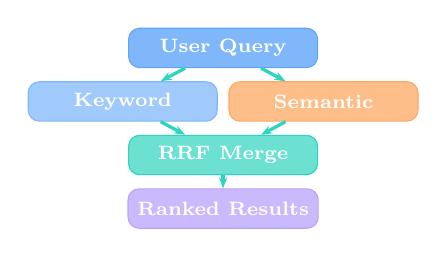
\begin{tikzpicture}[
    box/.style={rectangle, rounded corners=4pt, minimum height=0.5cm, text centered, font=\scriptsize\bfseries\color{white}, minimum width=2.4cm},
    arr/.style={-{Stealth[length=4pt]}, very thick, accentTeal},
    scale=0.85
]
\node[box, fill=accentBlue!80, draw=accentBlue] (q) at (0,0) {User Query};
\node[box, fill=accentBlue!60, draw=accentBlue!80] (bm) at (-1.5,-0.8) {Keyword};
\node[box, fill=accentOrange!60, draw=accentOrange!80] (kn) at (1.5,-0.8) {Semantic};
\node[box, fill=accentTeal!70, draw=accentTeal] (rrf) at (0,-1.6) {RRF Merge};
\node[box, fill=accentPurple!60, draw=accentPurple!80] (res) at (0,-2.4) {Ranked Results};
\draw[arr] (q) -- (bm);
\draw[arr] (q) -- (kn);
\draw[arr] (bm) -- (rrf);
\draw[arr] (kn) -- (rrf);
\draw[arr] (rrf) -- (res);
\end{tikzpicture}
\end{exampleblock}

\begin{block}{Kết quả (industry reports)}
{\small
\begin{itemize}
    \item Conversion rate tăng \textbf{15--25\%}
    \item Zero-result queries giảm \textbf{40--60\%}
\end{itemize}
}
\end{block}

\end{column}
\end{columns}
\end{frame}

% ── Case Study 2: Our Project ──
\begin{frame}{Case Study 2: Academic Paper Search (Project của nhóm)}

\begin{columns}[T]
\begin{column}{0.48\textwidth}

\begin{block}{Bối cảnh tương tự}
{\scriptsize \textbf{1.2 triệu} bài báo CS từ arXiv. Cùng 3 loại query:}
\end{block}

\vspace{0.05cm}

{\scriptsize
\textbf{Exact:} ``BERT fine-tuning'' \\
\textbf{Semantic:} ``methods to detect fake images'' \\
\textbf{Mixed:} ``transformer for NLP tasks''
}

\vspace{0.1cm}

\begin{exampleblock}{Kết quả NDCG@10 (30 queries)}
{\scriptsize
\begin{tabular}{l c c c}
\toprule
& \textbf{Exact} & \textbf{Sem.} & \textbf{Mixed} \\
\midrule
Từ khóa (BM25) & 0.64 & 0.68 & 0.70 \\
Ngữ nghĩa (kNN) & 0.66 & 0.66 & 0.68 \\
\rowcolor{highlightRow}
\textcolor{accentTeal}{\textbf{Kết hợp (Hybrid)}} & \textcolor{accentTeal}{\textbf{0.98}} & \textcolor{accentTeal}{\textbf{0.95}} & \textcolor{accentTeal}{\textbf{0.98}} \\
\bottomrule
\end{tabular}
}
\end{exampleblock}

\end{column}
\begin{column}{0.48\textwidth}

\begin{alertblock}{So sánh với E-commerce}
{\scriptsize
\begin{tabular}{l l l}
\toprule
\textbf{Khía cạnh} & \textbf{E-commerce} & \textbf{Academic} \\
\midrule
Quy mô & 100M+ & 1.2M \\
Query & đa dạng & chuyên ngành \\
Embedding & product desc & title+abstract \\
Metric & CTR, CVR & NDCG, MRR \\
\bottomrule
\end{tabular}
}
\end{alertblock}

\vspace{0.05cm}

\begin{block}{Key Insight}
{\scriptsize Overlap (Keyword $\cap$ Semantic) chỉ \textbf{1.5/10}\\
$\to$ Hai phương pháp tìm kết quả \textbf{rất khác nhau}\\
$\to$ Hybrid kết hợp cả hai $\to$ NDCG tăng từ ${\sim}0.67$ lên ${\sim}0.97$\\[3pt]
\textbf{Tech:} ES 8.12, MiniLM-L6-v2, RRF k=60, FastAPI, React}
\end{block}

\end{column}
\end{columns}
\end{frame}

% ============================================================
% SECTION 6
% ============================================================
\section{Kết luận \& Xu hướng}

\begin{frame}{Key Takeaways \& Xu hướng tương lai}
\begin{columns}[T]
\begin{column}{0.46\textwidth}

\begin{exampleblock}{1. Keyword $\neq$ Semantic}
{\scriptsize Hai paradigm \textbf{bổ sung nhau}, không thay thế. Tìm kiếm từ khóa giỏi exact terms, tìm kiếm ngữ nghĩa giỏi paraphrase.}
\end{exampleblock}

\vspace{0.05cm}

\begin{exampleblock}{2. RRF: Đơn giản, hiệu quả}
{\scriptsize Parameter-free, không cần normalize. Là mặc định của Elasticsearch, Azure AI Search.}
\end{exampleblock}

\vspace{0.05cm}

\begin{exampleblock}{3. Tìm kiếm xấp xỉ giải bài toán scale}
{\scriptsize HNSW, IVF, ScaNN biến đổi $O(N) \to O(\log N)$, hỗ trợ tìm kiếm trên hàng triệu---tỷ vectors.}
\end{exampleblock}

\end{column}
\begin{column}{0.50\textwidth}

\begin{block}{Xu hướng 2024--2026}
\begin{itemize}
    \item \textbf{RAG}: Hybrid Search + LLM\\
    {\scriptsize$\to$ ChatGPT trả lời từ dữ liệu riêng}
    \item \textbf{Multi-stage Retrieval}:\\
    {\scriptsize Hybrid (fast) $\to$ Cross-Encoder (accurate)}
    \item \textbf{Learned Sparse}: SPLADE, ColBERT\\
    {\scriptsize$\to$ Kết hợp sparse + dense trong 1 model}
    \item \textbf{Multimodal Search}:\\
    {\scriptsize Text + image + audio cùng lúc}
    \item \textbf{Vector Databases}:\\
    {\scriptsize Pinecone, Weaviate, Qdrant, Milvus}
\end{itemize}
\end{block}

\vspace{0.05cm}
{\scriptsize\textcolor{accentTeal}{Hybrid Search là \textbf{kiến trúc nền tảng} cho thế hệ ứng dụng AI tiếp theo.}}

\end{column}
\end{columns}
\end{frame}

% ── Q&A ──
\begin{frame}[plain]
\begin{center}

\vspace{2cm}
{\Huge\textbf{\textcolor{accentTeal}{Cảm ơn!}}}

\vspace{0.5cm}
{\LARGE Q \& A}

\vspace{1cm}

{\large\textcolor{textLight}{Hybrid Search: Keyword + Semantic + Rank Fusion}}\\
\vspace{0.2cm}
{\small\textcolor{textMuted}{Group 11 --- CO5135 Big Data --- HCMUT, HK252}}

\vspace{1cm}
{\small\textcolor{textMuted}{Source: \url{https://github.com/kinggiaan/Big-Data}}}

\end{center}
\end{frame}

% ============================================================
% BACKUP SLIDES
% ============================================================
\appendix
\section{Phần phụ lục (Appendix)}

\begin{frame}{Backup: Latency \& Storage Benchmark}
\begin{columns}[T]
\begin{column}{0.50\textwidth}

\begin{block}{Latency qua các quy mô}
\centering
{\scriptsize
\begin{tabular}{l *{6}{c}}
\toprule
\multirow{2}{*}{\textbf{Method}} & \multicolumn{2}{c}{\textbf{100k}} & \multicolumn{2}{c}{\textbf{500k}} & \multicolumn{2}{c}{\textbf{1.2M}} \\
\cmidrule(lr){2-3} \cmidrule(lr){4-5} \cmidrule(lr){6-7}
& P50 & P95 & P50 & P95 & P50 & P95 \\
\midrule
BM25 & 15 & 56 & 21 & 37 & 71 & 153 \\
kNN & 13 & 34 & 20 & 41 & 191 & 1206 \\
\rowcolor{highlightRow}
\textcolor{accentTeal}{Hybrid} & \textcolor{accentTeal}{30} & \textcolor{accentTeal}{53} & \textcolor{accentTeal}{42} & \textcolor{accentTeal}{62} & \textcolor{accentTeal}{99} & \textcolor{accentTeal}{156} \\
\bottomrule
\end{tabular}
}
{\scriptsize\textcolor{textLight}{(đơn vị: ms)}}
\end{block}

\vspace{0.1cm}
{\small
\begin{itemize}
    \item kNN P95=1206ms ở 1.2M: HNSW cold start
    \item Sau warm cache: Hybrid chỉ \textbf{99ms}
\end{itemize}
}

\end{column}
\begin{column}{0.46\textwidth}

\begin{block}{Storage Scaling}
\centering
{\scriptsize
\begin{tabular}{l c c c}
\toprule
\textbf{Scale} & \textbf{Docs} & \textbf{JSONL} & \textbf{ES Index} \\
\midrule
100k & 100K & 917 MB & 860 MB \\
500k & 500K & 4.6 GB & 4.3 GB \\
1.2M & 1.2M & 12 GB & 11.9 GB \\
\bottomrule
\end{tabular}
}
\end{block}

\vspace{0.1cm}
{\small
\begin{itemize}
    \item \textbf{87\%} dung lượng là vector (HNSW graph)
    \item Tăng trưởng tuyến tính theo docs
    \item Mỗi vector: $384 \times 4 = 1{,}536$ bytes
\end{itemize}
}

\end{column}
\end{columns}
\end{frame}

\begin{frame}{Backup: BM25 --- Ví dụ tính điểm step-by-step}

\textbf{Query:} ``attention mechanism'' \quad {\small Corpus: 1.2M papers}

\vspace{0.3cm}

\begin{columns}[T]
\begin{column}{0.50\textwidth}

\begin{block}{Bước 1: Analyze query}
{\scriptsize
\texttt{attention mechanism}\\
$\downarrow$ Analyzer: lowercase $\to$ stemming\\
$\to$ Tokens: \texttt{[attent, mechan]}
}
\end{block}

\begin{block}{Bước 2: Tra Inverted Index}
{\scriptsize
\texttt{attent} $\to$ $\{D_{42}, D_{107}, D_{1580}, ...\}$\\
\texttt{mechan} $\to$ $\{D_{42}, D_{305}, D_{8921}, ...\}$\\
Giao tập $\to$ $\{D_{42}, ...\}$
}
\end{block}

\end{column}
\begin{column}{0.46\textwidth}

\begin{exampleblock}{Bước 3: Tính BM25}
{\scriptsize Với $D_{42}$ (``Attention Is All You Need''):
\begin{itemize}
    \item TF(attent, title) = 1
    \item IDF(attent) = 4.2 {\tiny(từ hiếm)}
    \item Title boost $\times 2$
    \item $\Rightarrow$ Score = \textbf{12.8}
\end{itemize}
}
\end{exampleblock}

\vspace{0.15cm}

\begin{alertblock}{Khi BM25 thất bại}
{\scriptsize ``methods to detect fake images'' \\
$\to$ Không match ``deepfake detection'' \\
vì \textbf{0 từ khóa chung!} Cần Tìm kiếm ngữ nghĩa.}
\end{alertblock}

\end{column}
\end{columns}
\end{frame}

\end{document}
